\section{Background}
\label{sec:background}

Un metodo efficace per l'astrazione del concetto consiste 
in una rappresentazione tramite un reticolo, in inglese ``lattice''.

\begin{definition}[Reticolo]
    Un reticolo è un insieme di punti o nodi (siti) connessi da archi (legami), 
    ciascuno in grado di identificare un ordine locale per il riconoscimento dei primi vicini.
\end{definition}

In un reticolo in cui vale questa relazione è possibile descrivere due tipi di percolazione: 
\begin{itemize}
    \item percolazione di legame;
    \item percolazione di sito.
\end{itemize}

\begin{figure}
    \centering
    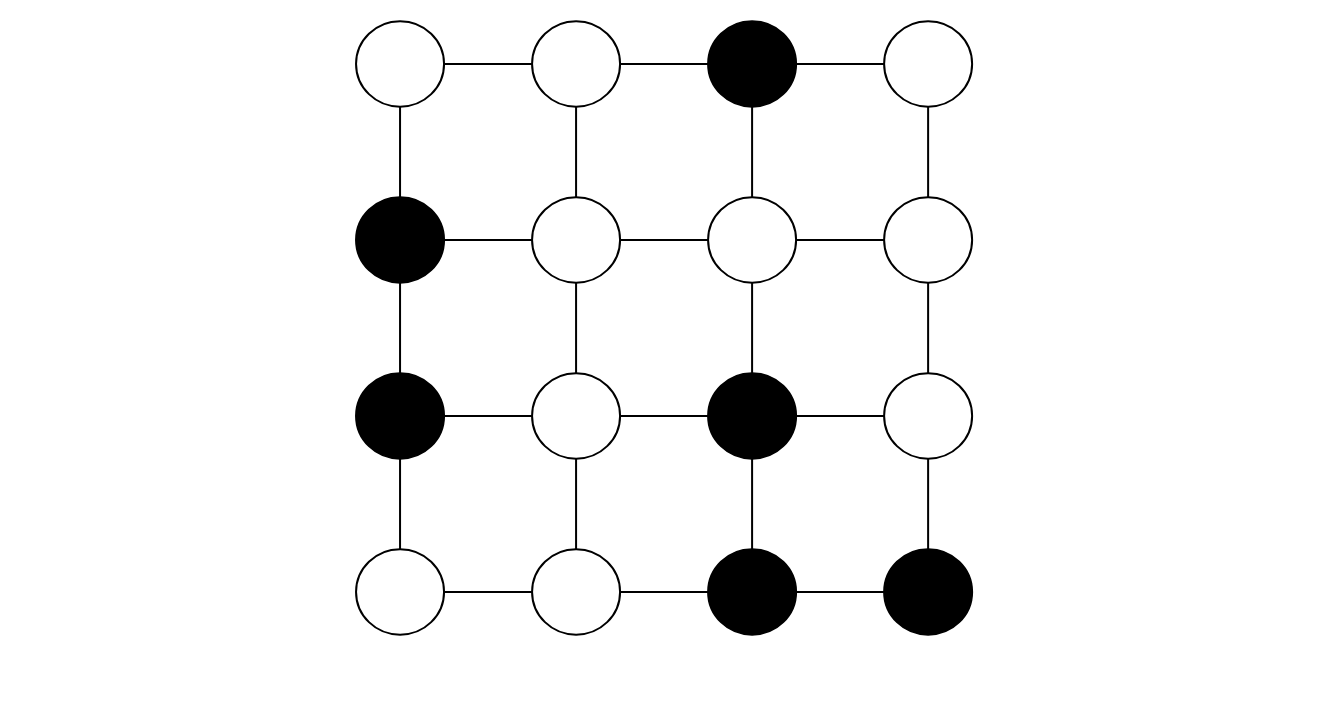
\includegraphics[width=0.4\textwidth]{2D-lattice}
    \caption{Esempio di reticolo quadrato bidimensionale}
    \label{fig:ex-lattice}
\end{figure}

\subsection*{Percolazione di legame}
È la prima versione del modello fornita da Broadbent e Hammersley \cite{broadbent}.
Ogni legame ha probabilità $p$ di essere ``aperto'', quindi
probabilità $1-p$ di essere ``chiuso''. Se due siti formano un legame aperto, vi è un 
collegamento diretto, quindi possono essere considerati primi vicini. Al contrario, un 
legame chiuso elimina il collegamento tra i due siti nel reticolo.
In questa versione, ``avviene percolazione'' se esiste un percorso (insieme di legami) 
che attraversa l'intero reticolo. La percolazione può verificarsi 
sia in verticale (alto-basso) sia in orizzontale (sinistra-destra).

\subsection*{Percolazione di sito}
In questo modello ogni sito ha una probabilità $p$ di essere occupato, di conseguenza
probabilità $1-p$ di essere vuoto. In figura \ref{fig:ex-lattice} viene mostrato un 
reticolo bidimensionale quadrato con nodi occupati (neri) e vuoti (bianchi). Questo è 
il modello che verrà utilizzato per lo studio dell'argomento e dei vari algoritmi, verrà
dunque approfondito più in dettaglio nella sezione \ref{sec:implementazione}.

\subsection*{Soglia di percolazione}
I due modelli appena introdotti rappresentano soluzioni valide per lo studio 
del fenomeno. Nonostante la somiglianza, vi sono differenze concettuali che si 
riflettono anche nel calcolo di alcuni valori caratteristici \cite{weisstein-bond,weisstein-site,weisstein-threshold}.

\begin{definition}[Soglia di percolazione]
    Sia $L$ un reticolo di taglia infinita\footnote{Con il termine ``infinito'' 
    si fa riferimento all'estensione intuitiva delle varie proprietà della struttura,
    come avviene in matematica per il concetto di \textit{limite all'infinito}.}. 
    Sia $p$ la probabilità di occupazione dei siti o di apertura 
    dei legami, a seconda del modello scelto.
    La soglia di percolazione per $L$ è definita come la 
    probabilità $p_c$ tale per cui:
    \begin{itemize}
        \item se $p > p_c$, allora vi è percolazione;
        \item se $p < p_c$, allora non vi è percolazione.
    \end{itemize}
\end{definition}

\begin{figure}
    \centering
    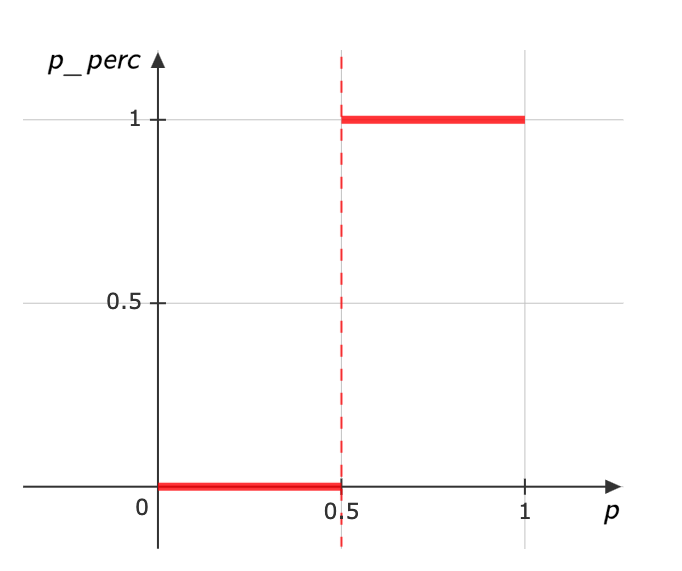
\includegraphics[width=0.4\textwidth]{threshold.png}
    \caption{Grafico relativo alla soglia di percolazione ($p_c=0.5$)}
    \label{fig:threshold}
\end{figure}

È possibile visualizzare il concetto di soglia nel grafico mostrato in 
figura \ref{fig:threshold}. Nel grafico, l'asse delle ascisse è associato alla 
probabilità $p$, mentre l'asse delle ordinate è associato alla probabilità
che avvenga percolazione $p_perc$.
Nei casi reali, ovvero per reticoli di taglia finita, non è possibile stabilire
un'affermazione così forte. 

Ciò che è possibile preservare dalla definizione 
è che esiste un \textbf{punto critico} $p_c$ relativo alla probabilità $p$, oltre 
al quale è molto probabile che avvenga percolazione e, al contrario, al di sotto
del quale è molto improbabile che questo si verifichi.

\begin{table}[ht!]
    \centering
    \begin{tabular}{lcc}
    \toprule
    \textbf{Lattice} & \textbf{\(p_c\) (Site)} & \textbf{\(p_c\) (Bond)} \\
    \midrule
    Cubic (body-centered) & 0.246    & 0.1803    \\
    Cubic (face-centered) & 0.198    & 0.119     \\
    Cubic (simple)        & 0.3116   & 0.2488    \\
    Diamond               & 0.43     & 0.388     \\
    Honeycomb             & 0.6962   & 0.65271*  \\
    4-Hypercubic          & 0.197    & 0.1601    \\
    5-Hypercubic          & 0.141    & 0.1182    \\
    6-Hypercubic          & 0.107    & 0.0942    \\
    7-Hypercubic          & 0.089    & 0.0787    \\
    Square                & 0.592746 & 0.50000*  \\
    Triangular            & 0.50000* & 0.34729*  \\
    \bottomrule
    \end{tabular}
    \caption{Punti critici (\(p_c\)) per reticoli regolari.}
    \label{tab:percolation}
\end{table}

In letteratura sono presenti diversi studi sulle caratteristiche di vari 
reticoli e i rispettivi valori di soglia. La tabella \ref{tab:percolation}
mostra i punti critici per diversi reticoli regolari, ovvero in cui il reticolo è composto
da elementi ripetuti della stessa forma. La colonna \textbf{Lattice} indica la forma 
del reticolo, mentre le colonne \textbf{Site} e \textbf{Bond} distinguono i valori 
in percolazione di sito e di legame, rispettivamente \cite{stauffer-threshold}.
Vi è una lieve, ma evidente, discrepanza tra i valori nelle due colonne.
In generale, la rappresentazione tramite occupazione dei siti è considerata
più generica rispetto alla sua controparte, questo perché la percolazione di legame
può essere riformulata in termini di percolazione di sito, 
ma non si può affermare il contrario.

